\documentclass[11pt]{article}
\usepackage[margin=0.85in]{geometry}
\usepackage{fontspec}\setmainfont{Times New Roman}
\usepackage{graphicx,booktabs,array,placeins,microtype}
\usepackage[hidelinks]{hyperref}
\usepackage{caption}
\setlength{\emergencystretch}{3em}
\setlength{\parskip}{5pt}
\title{Computational assessment of EBV-self peptide similarities across HLA class II contexts}
\author{}\date{}
\begin{document}\maketitle
\begin{abstract}
Over time, researchers have noticed a connection between patients who were diagnosed with multiple sclerosis and noted that over 99\% of patients have had EBV in the past \cite{bjornevik}. Therefore, molecular mimicry between viral and human antigens is one proposed cause of this observed association. In this study, computational analysis was used to identify the number of prospective pairs from 6,400 allele-specific EBV-self peptide pairs to 8 candidate pairs, of which 6 were placed on hold due to evidence gaps for experimental validation. This pipeline used epitopes from EBV and human myelin-associated proteins curated from IEDB and UniProt across 4 HLA alleles to find viable molecular mimicry pairs for experimental validation through the use of register-aware sequence similarity, binding register similarity, HLA-binding predictions, and AlphaFold 3 structure modeling. Through the analysis based on BLOSUM62 on allele-bound sequences, 2 potential pairs of BALF5-TALDO1 in HLA-DRB1*15:01 (14/1600) and HLA-DRB1*13:03 (13/1600) were found and explored further. In each pair, a peptide derived from BALF5, an EBV protein involved in DNA replication, had a computational similarity to a peptide derived from TALDO1 (transaldolase), a metabolic enzyme. Several other methods were attempted such as electrostatic comparison which failed its predefined control benchmark and TCR docking which didn’t consistently recover docking poses. These findings were able to support BALF5-TALDO1 as a mimicry candidate, however further research into T-cell cross-reactivity and natural presentation is needed.

\end{abstract}
\FloatBarrier\section{Introduction}
Multiple sclerosis (MS) is an autoimmune disease that can cause a degeneration of motor, sensory, visual, and cognitive abilities and is caused by immune-mediated damage that affects myelin sheaths in the brain, spinal cord, and optic nerves. A myelin sheath covers the neuron's axon and acts as plastic insulation on an electrical wire. It is a key component for function of the central and peripheral nervous system \cite{ninds}.

In 2022, Bjornevik et al. studied a cohort of more than 10 million US military personnel; 955 of whom developed MS. According to Bjornevik et al.’s data analysis, MS risk increased approximately 32-fold following EBV infection. Meanwhile, cytomegalovirus was found to have no comparable increase in MS risk in Bjornevik et al.’s study. The biomarker (serum neurofilament light chain) of nerve-fiber injury after EBV seen by Bjornevik et al showed that observed serum neurofilament light only increased after EBV infection, indicating that EBV may precede detectable neurological injury. \cite{bjornevik} In 2022, Lanz et al. identified an antibody from an MS patient that recognized both EBV EBNA1 and the human CNS protein GlialCAM. This evidence supports the theory that molecular mimicry is the source of the connection between EBV and MS. \cite{lanz}

Previous studies like the one conducted by Lanz et al. in 2022 identified cross-reactive antibodies \cite{lanz}, however comprehensive mapping of T-cell cross-reactivity remains incompletely defined. T-cell receptors (TCRs) recognize a specific peptide presented within the binding groove of a human leukocyte antigen (HLA) molecule rather than the peptide alone. Consequently, sequence-only comparisons of peptide-MHCs (pMHC) do not directly define the HLA binding aspect of immune recognition. Furthermore, different HLA alleles show distinct structural preferences, changing both the pMHC binding affinity and the specific binding register, the placement of the 9-amino acid core within the HLA groove. This binding register directly determines which amino acid residues are anchor residues and which are TCR contact residues.

To address this gap in research, the computational pipeline developed in this study provides a filtering mechanism. By integrating peptide-HLA binding predictions, register-aware sequence alignments, and predicted three-dimensional peptide-HLA structures, the pipeline was able to prioritize a small subset of viral-self peptide pairs prior to laboratory testing. Although predicted structural or sequence resemblance doesn’t guarantee stable cell-surface presentation or functional T-cell activation in vivo, the models describe predicted similarities between pMHCs rather than actual experimentally confirmed registers.

\FloatBarrier\section{Materials and Methods}
This study describes a computational prioritization pipeline designed to identify high-interest Epstein-Barr virus (EBV)-human self-peptide candidate pairs for subsequent experimental peptide-HLA binding and binding register validation. This computational workflow integrated predicted HLA binding affinities, register-aware sequence alignments, structural modeling, and downstream evidence reviews. However, these computational predictions alone do not establish natural processing and presentation in vivo, surface pMHC stability, or T-cell receptor (TCR) recognition and functional cross-reactivity.

In our computation pipeline, an EBV repertoire was curated from the Immune Epitope Database (IEDB) \cite{iedb} and experimental filters were used to identify linear human-targeted epitopes. For human self-proteins, the pipeline selected human myelin-associated and central nervous system (CNS) proteins from both IEDB records and UniProt reference proteomes \cite{uniprot}. To ensure quality, the pipeline removed duplicate peptide sequences, peptides with invalid length (<9 AA or >25 AA), and sequences containing nonstandard or ambiguous amino-acid single-letter codes (i.e. X, B, Z). Finally, it filtered and screened the peptides through NetMHCIIpan and created a final universe of 6400 allele-specific peptide pairs.

In the pipeline, analysis was limited to HLA-DRB1*03:01, HLA-DRB1*08:01, HLA-DRB1*13:03, and HLA-DRB1*15:01. To prevent biologically invalid results, each HLA allele was evaluated independently, meaning pMHCs from one allele were never compared with pMHCs from another allele. Furthermore, to ensure consistency, the HLA-DRA*01:01 was part of every pMHCs model in the pipeline.

For the first stage of analysis the pipeline predicted binding affinities and percentile ranks of the peptide-HLA class II using NetMHCIIpan-4.3 \cite{netmhc} for the 15-mer windowed peptide frame. In order to be a valid pair within the same allele, both the viral peptide and the human self-peptide were required to meet a predicted binding threshold of $\leq$5.0\% for stage one and $\leq$20\% for stage two to be considered a valid candidate. To maintain data integrity, peptides were marked as computational predicted binders unless the IEDB data specified experimental binding assay records.

For the second stage of analysis, the binding-register alignment of all pairs was analyzed. The binding register is defined as the 9-residue core (referred to as P1 through P9) positioned within the open-ended HLA class II binding groove. By using the core assignments determined by the NetMHCIIpan-4.3 algorithm, the pipeline assigned a predicted binding register and verified these registers against independent core assignment algorithms. These disagreements between independent prediction algorithms were logged as a categorical binary status for each peptide. To completely evaluate the binding register, major anchor residues (P1, P4, P6, P9) were evaluated for HLA stability, whereas TCR contact residues (P2, P3, P5, P7, P8) were isolated for TCR contact analysis.

Alongside binding register similarity, sequence similarity was also calculated using the BLOSUM62 substitution matrix \cite{blosum}. Since the entire sequence with the exception of the peptide chain is identical in each allele-bound pair and HLA anchor residues aren’t evaluated by the TCR upon contact, sequence similarity was restricted strictly to the predicted TCR-contact residue positions (P2, P3, P5, P7, P8) derived from the aligned 9-residue binding cores. In the scoring interface, higher substitution matrix alignment scores indicated greater structural and physicochemical resemblance at the potential TCR interface. To normalize ranking, percentile rankings were calculated independently within each specific HLA allele cohort.

In the pipeline, heterotrimeric pMHC complexes (HLA-DRA + HLA-DRB1 + target peptide) were modeled using Alphafold 3 web server \cite{af3} across five random seed iterations per pMHC. The completeness of each model was evaluated through a quality analysis framework that verified coordinate completion, stereochemical geometry, and atom-level confidence metrics (pLDDT > 80). Specifically, since the entire pMHC consists of very well-defined chains, the pipeline isolated the peptide alphafold numbers to prevent any overshadowing by the other chains in confidence metrics. Structural deviation between peptides was quantified using backbone root-mean-square-deviation (RMSD) calculated over the Ca atoms of the defined 9-residue binding core following alignment of the HLA-a1 and b1 domain helices. To prevent overstating the bounds of our claims, AF3 outputs were treated strictly as predicted models rather than experimental coordinates and were therefore both consistently evaluated against experimental structures from PDB and were analyzed independently of TCR docking simulations.

After the list of 6400 allele-specific pairs was narrowed down to just 8 high-ranking candidates, the high-ranking pairs went through a standardized manual evidence audit. In this audit, the predicted binding affinity, register agreement across predictors, IEDB origin provenance, mass spectrometry immunopeptidome detection evidence, viral sequence conservation, and human self-protein tissue expression rarity were evaluated. Based on this multi-omic evidence audit, each pair was categorized as either high priority, medium priority, or hold. This placed six candidates on hold due to missing immunopeptidomic presentation or register discrepancies, while classifying two candidates (BALF5\textsubscript{627-641} and TALDO1\textsubscript{108-122} (DRB1*13:03) and -TALDO1\textsubscript{216-230} (DRB1*15:01)) as Medium Priority.

To ensure consistency with literature, the model used a novel method of positive calibration. The published BALF5 276-290 vs MBP 85-99 cross-reactive benchmark \cite{lang} was used to serve as a structural calibration reference for our ranking system. Because this control pair spans HLA-DRB5*01:01 (BALF5) and HLA-DRB1*15:01 (MBP), it was categorized as a DR15 haplotype-level control system rather than a single-allele comparison. To ensure consistency, redundant or overlapping peptide assay entries from IEDB were merged into single reference records before threshold benchmarking was performed.

Alongside the main methods of register-aware sequence similarity and binding register physicochemical similarity, several other methods were explored and were abandoned due to failure of controls. An attempt was made to use Poisson-Boltzmann electrostatic surface potential comparison, but the results were excluded from primary candidate ranking because the electrostatic similarity scoring failed to discriminate between the positive calibration control benchmark. Additionally, TCRmodel2 \cite{tcr} docking simulations were tried to evaluate pMHC-TCR complex pose recovery against solved structures. However, since the pose recovery didn’t consistently meet the RMSD convergence criteria (<2.5 A), the docking outputs were classified strictly as supplemental observations.

Throughout the pipeline, a high degree of reproducibility was maintained through thorough documentation of the entire process is found in our GitHub library. In the Github repository, The software environments, random seeds, input logs, and dataset checksums (SHA-256) are all retained to maintain full reproducibility. Furthermore, the ranking algorithms were completely deterministic. For example, ties in sequence similarity were systematically broken using HLA binding affinity percentile ranks determined by NetMHCIIpan. Additionally, for unevaluated or incomplete evidence in public databases, those data points were marked as “Not Reported” rather than negative. Finally, an effort was made to make sure not to fit nominal p-values, false discovery rates (FDR), or probabilistic “mimicry probability”, as formal statistical distribution models in the computational rankings.

\begin{figure}[htbp]\centering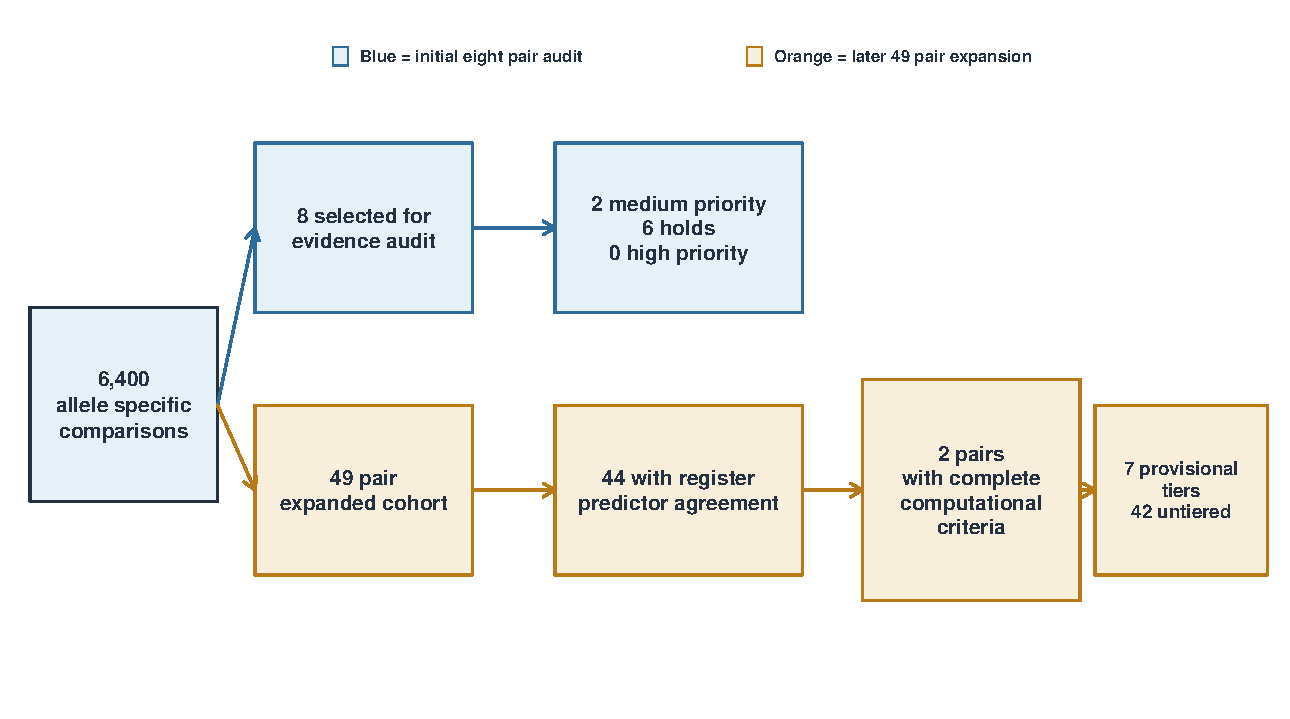
\includegraphics[width=0.95\linewidth]{figures/figure1.pdf}\caption{Multi-stage computational screening and evidence-audit workflow for EBV-self peptide pairs}\end{figure}
\FloatBarrier\section{Results}
\subsection{Initial sequence comparisons across four HLA alleles}
Initially, a total of 6,400 allele-specific peptide pair comparisons were evaluated across the four target alleles, separated evenly into 1,600 pairs for each allele batch (HLA-DRB1-03:01, HLA-DRB1*08:01, HLA-DRB1*13:03, and HLA-DRB1*15:01). Alongside binding register metrics, sequence similarity metrics were subsequently derived across predicted TCR-contact residues (P2, P3, P5, P7, P8). Across all four target alleles, the resulting score distributions exhibited marked rightward skewing, with a minimal subset of candidate pairs demonstrating elevated structural and sequence similarity at potential TCR contact sites (Figure 2). However, it is important to note that the scores reflected a relative physiochemical substitution matrix resemblance, not a percentage identity or a clear probability of cross-reactivity.

The pair EBNA1\textsubscript{87-101}- ANO2\textsubscript{79-93} was the top sequence rank (score 0.522) in two distinct allele contexts: HLA-DRB1*08:01 and HLA-DRB1*15:01. In contrast, the remaining allele cohorts were led by different pairs: EBNA2\textsubscript{136-150}-MOG\textsubscript{97-109}was the top pair for HLA-DRB1*03:01 (score 0.480), and EBNA3B\textsubscript{139-153}-MOG\textsubscript{221-235} was the top pair for HLA-DRB1*13:03 (score 0.485). Some other high-ranking pairs that included the BLLF1\textsubscript{65-75}-PLP1\textsubscript{140-152} (rank 4, HLA-DRB1*13:03) and BLLF1\textsubscript{65-75}-CLDN11\textsubscript{193-207} (rank 6, HLA-DRB1*15:01)

\begin{table}[htbp]\centering\footnotesize
\caption{Ranking of top pairs for each allele based on sequence-based analysis}
\setlength{\tabcolsep}{3pt}\renewcommand{\arraystretch}{1.25}
\begin{tabular}{p{0.112\textwidth}p{0.27\textwidth}p{0.27\textwidth}p{0.279\textwidth}}
\toprule
HLA-DRB1 Allele & Rank 1 Pair (Score) & Rank 2 Pair (Score) & Rank 3 Pair (Score) \\
\midrule
*03:01 & EBNA2\textsubscript{136-150}- MOG\textsubscript{97-109} (0.48) & BNRF1\textsubscript{37-51}- CLDN11\textsubscript{193-207} (0.44) & BALF4\textsubscript{103-116} - CRYAB\textsubscript{1-15} (0.41) \\
*08:01 & EBNA1\textsubscript{87-101}- ANO2\textsubscript{79-93} (0.522) & BLLF1\textsubscript{65-75}-PLP1\textsubscript{140-152} (0.42) & BZLF1\textsubscript{198-210} - MAG\textsubscript{612-626} (0.391) \\
*13:03 & EBNA3B\textsubscript{139-153} - MOG\textsubscript{221-235} (0.49) & BNRF1\textsubscript{37-51}- CLDN11\textsubscript{193-207} (0.44) & BARF1\textsubscript{1-15} - MAG\textsubscript{1-15} (0.44) \\
*15:01 & EBNA1\textsubscript{87-101}- ANO2\textsubscript{79-93} (0.522) & EBNA3B\textsubscript{139-153}-MOG\textsubscript{221-235} (0.49) & BALF4\textsubscript{575-589} - CNP\textsubscript{1-15} (0.43) \\
\bottomrule\end{tabular}\end{table}
In the computational pipeline’s sequence similarity ranking results, the BALF5\textsubscript{627-641} peptide paired with the human TALDO1\textsubscript{108-122} peptide achieved a similarity score of 0.281 in HLA-DRB1*13:03, ranking 13 of 1600 pairs. Similarly, the BALF5\textsubscript{627-641} viral peptide paired with the human TALDO1\textsubscript{216-230} peptide achieved a similarity score of 0.314 in HLA-DRB1*15:01, ranked 14 of 1600.

However, it is important to note that these two comparisons involve different human peptide regions rather than one identical pair. That said, both pairings showed a 40.0\% sequence identity (2/5 residues) across the TCR-contact positions (P2, P3, P5, P7, P8), with a full-core identity of \textasciitilde{}22.2\% (2/9) in *13:03 and 33.3\% (3/9 residues) in *15:01. Although, as seen above, several other candidates received higher primary sequence similarity scores, the BALF5-TALDO1 pairing was prioritized later on based on multi-layered evidence in future steps and in literature. Furthermore, it is important to note that relative rankings shifted by a significant amount when evaluated under alternative scoring formulations. When using full-core BLOSUM62 scoring, the HLA-DRB1*13:03 BALF5\textsubscript{627-641}-TALDO1\textsubscript{108-122} candidate dropped to rank 173, while the HLA-DRB1*15:01 candidate jumped to rank 3. Conversely, under the strict physiochemical mismatch scoring, the *13:03 candidate placed at rank 29, while the *15:01 candidate fell to rank 453. Finally, to preserve biological validity rather than breaking ties for a clean ranking, identical score ties were broken by binding affinities determined by the NetMHCIIpan.

\begin{figure}[htbp]\centering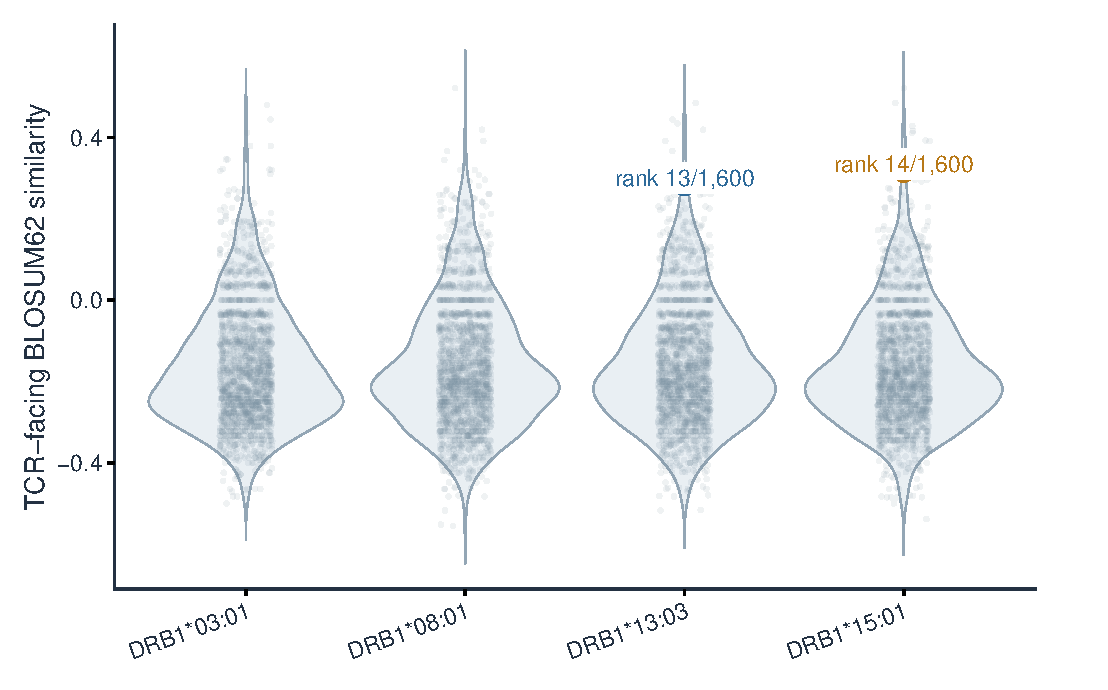
\includegraphics[width=0.95\linewidth]{figures/figure2.pdf}\caption{sequence rankings Distribution of primary TCR contact sequence similarity scores across four HLA-DRB1 alleles}\end{figure}
\FloatBarrier
\subsection{Initial Eight-Candidate Evidence Review}
The next stage of the computational pipeline was a targeted review of the evidence of a panel of eight preselected candidate pairs yielding two medium-priority pairs, six holds, and zero high priority pairs (Figure 3)


\begin{figure}[htbp]\centering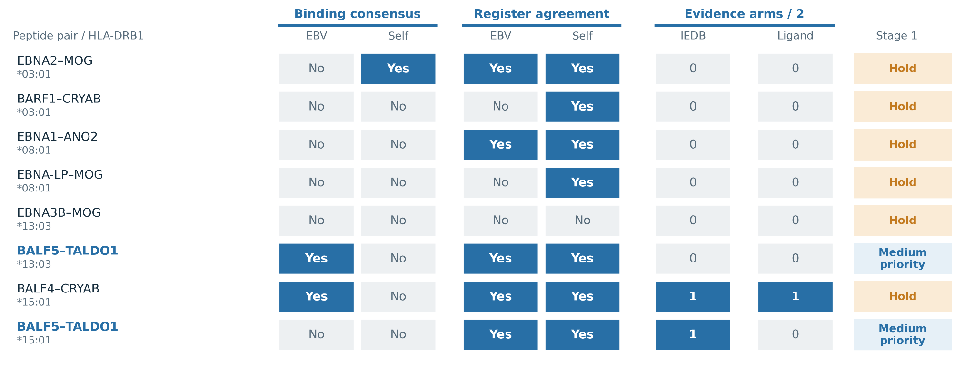
\includegraphics[width=0.95\linewidth]{figures/figure3.pdf}\caption{Initial eight-candidate evidence review across multiple validation layers}\end{figure}
\FloatBarrier
The two pairs that were classified as medium priority were the HLA-DRB1*13:03 (BALF5\textsubscript{627-641}-TALDO1\textsubscript{108-122}) and HLA-DRB1*15:01 (BALF5\textsubscript{627-641}-TALDO1\textsubscript{216-230}) candidates.

Both the medium priority BALF5-TALDO1 candidates exhibited a core register agreement across the prediction methods included in the initial review. However, it is important to note that the evaluation of these registers is all speculative, as experimental work has not confirmed these registers. That being said, neither context satisfied full-binding consensus criteria for HLA-anchor sequences with NetMHCIIpan. For the HLA-DRB1*13:03 candidate, the viral peptide arm met the minimum percentile to be considered a proper binder, while the self-peptide did not match up well enough with HLA-DRB1*13:03 according to the tool. On the other hand, in the HLA-DRB1*15:01 candidate, neither the self-peptide nor the viral peptide met the binding criteria for NetMHCIIpan. These binding affinity thresholds reflect the initial review step, as subsequent predictor outputs yielded different scores.

Finally, no corroborating evidence was found with public experimental evidence, such as mass spectrometry, eluted ligand records in the IEDB or immunopeptidome repositories sourced from PRIDE \cite{pride}, for either self-peptides.

The remaining six reviewed candidate pairs were placed on hold for the time being due to candidate-specific evidence gaps recorded by the computational pipeline, including discordance between predicted registers, failure of one of both peptides to satisfy the binding-consensus criteria, or absent public experimental assay records.

In summary, this review stage functioned as an initial evaluation of the eight pre-selected pairs and was independent of the parallel V3 structural-selection track. Also, these classifications were not static and were subsequently reevaluated through concentrated structural modeling and the expanded evidence review.

\subsection{Focused Structural Assessment of Predicted Binding Registers}

After completing the initial evaluation of the eight pre-selected pairs, the computational pipeline implemented several methods of structural assessment to assess possible gaps in the predicted binding registers. Specifically, the initial step of the review included a high resolution 3D structural modeling consisting of 13 submission jobs to alphafold 3 with five models each, totaling 65 structural models. Then, all generated models underwent verification checks for coordinate completeness, correct chain identifiers, and peptide sequence integrity.

Through the analysis, the computation pipeline yielded data that when observed, revealed allele specific patterns. In HLA-DRB1*13:03 (viral parent-nested median RMSD: 0.445), the 3D structures yielded consistent peptide coordinate recovery across independent seeds for viral peptides (BALF5\textsubscript{627-641}), but showed lower confidence scores and significant positional uncertainty for human self-peptide (TALDO1\textsubscript{108-122}) counterparts within the binding cleft. In HLA-DRB1*15:01 (viral RMSD 1.712, human RMSD: 0.888 A), most 3D structures displayed varying backbone poses among viral parent peptide models (BALF5\textsubscript{627-641}), but still demonstrated stable, consistent recovery of the proposed human 11-mer core window (TALDO1\textsubscript{216-230}) with moderate model confidence. Finally, in HLA-DRB5*01:01 (viral: 0.247 A), the 3D models showed disagreement between competing predicted registers for the human self-peptide (TALDO1\textsubscript{216-230}), with longer parent peptide modelling unable to stabilize or confirm either hypothesized placement.

In the analysis we also employed differing methods of peptide prediction in the modeling of the shorter 11-peptide sequence and the modelling of the complete 15-mer peptide sequence. In models of the short peptide sequence, results frequently converged, often reaching a consistent structural placement. However, in models of the entire 15-mer peptide sequence, this consistent placement was rarely recovered.

Finally, we calibrated the review pipeline to only focus on the model confidence in areas of interest like the binding register. Previously, the computational model would evaluate the global pMHC metrics (such as domain-level pLDDT), which can often obscure peptide uncertainty because the MHC chains are often more defined for the models than the exploratory peptide chains. After this calibration, the local confidence across the peptide binding groove was observed to be much lower. Furthermore, high register agreement across earlier sequence-based predictors didn’t amount to significant structural confirmation at the atomic backbone level.

\subsection{Cross Method Structural Reproducibility}
For the next stage of the computational model, cross-method structural reproducibility was implemented using PANDORA’s structural modelling tool coupled with MODELLER \cite{pandora,modeller}. For the first step, the PANDORA model was tested on its ability to model control models, passing its predefined benchmark of 120 models out of 120 models scored via stereochemical scoring and convergence criteria.

Next, an ensemble of 1200 structural models was generated and evaluated across the candidate peptides. Across the evaluation of these models, it was determined that across the candidate pool, 0 of the 10 evaluated peptides (0/10) in the randomly sampled dataset demonstrated support for the binding register that was expected (according to NetMHCIIPan) across both structural templates. In another attempt at cross-method structural reproducibility, a subsequent AlphaFold structural modeling dataset was used. The modeling dataset yielded 150 completed models with 30 completed jobs of 5 models each, with eight candidate pairs in the random sample having uncertain binding-register placement.

The implication of this finding is that the principal factor preventing meaningful structural comparison between the registers could be due to conformational instability and register drift within the proposed core windows across templates and replicates. This shows the register instability involved in structural modeling tools like Alphafold3 and Pandora/MODELLER and therefore the results of binding register indication should not be interpreted as evidence that localized electrostatic or charge alterations disrupted the binding.

\subsection{Expanded Assessment of 49 Candidate Pairs}
After the initial screening was determined to be excessively selective, the computational pipeline thereafter attempted to expand the sample by increasing the new cohort from 8 peptide pairs to 49 peptide pairs. These 49 candidate pairs were recovered from the near-miss list in the sequence similarity ranking. We then completed computational binding affinity and core-register prediction using NetMHCIIpan for all 98 peptides.

To ensure consistency in the data, the registers evaluated by NetMHCIIpan were evaluated against registers determined by MixMHC2pred \cite{mix2019,mix2023}. Across 49 peptide pairs, 44 pairs passed this stage, which demonstrates the high degree of computational agreement between the predictive models, rather than any experimentally confirmed structural placement within the HLA groove.

Next, only two of the remaining 44 pairs satisfied all evaluated binding and register criteria (<= 20 percentile). Both of the passing candidates corresponded to the BALF5\textsubscript{627-641}-TALDO1\textsubscript{108-122} and BALF5\textsubscript{627-641}-TALDO1\textsubscript{216-230} pairings in HLA-DRB1*13:03 and HLA-DRB1*15:01 respectively and in this expanded evaluation, the requirement of the models agreeing proved to be much more restrictive than the earlier barrier of reaching a register-predictor agreement.

In an attempt to ground the computational data with experimental data, targeted manual verification within the IEDB recovered a direct, experimentally confirmed positive binding record for the viral BALF5\textsubscript{627-641} peptide in the context of HLA-DRB1*15:01. However, the recovered assay only confirmed the viral peptide and didn’t confirm the self-peptide (TALDO1\textsubscript{216-230}) binding, stable presentation, or dual-reactive T cell-recognition.

After analysis that utilized sequence metrics, targeted assay verification, and subsequent PANDORA structural-template consistency, a differentiation provisional shortlist consisting of seven prioritized candidates. In the seven prioritized candidates, 1 was described as a strong-medium candidate, 2 were described as weak-medium candidates, and 4 were described as strong-low candidates. The remaining 42 candidates were left untiered to insufficient evidence to justify a priority ranking and detailed tier explanations are described in Section 3.6. Moreover, no pairs were classified as high-priority due to the unavailability to retrieve and analyze public immunopeptidome repositories.

\subsection{Secondary Provisional Classifications}
After the initial analysis of the 49-pair cohort, secondary evidence review was performed stratifying the candidates into distinct tiers. After that stratification was performed, one strong-medium pair, two weak-medium, and four strong-low candidates were determined, of which the 42 remaining pairs remained untiered. Under the criteria used by this review, no candidates qualified for a high-priority classification. That said, these assignments represent provisional evidence categories that were established under the criteria of the expanded review and are not equivalent to the categories used in the initial eight-candidate review.

\begin{table}[htbp]\centering\footnotesize
\caption{Candidate classification and evidence audit of the expanded 49-pair cohort}
\setlength{\tabcolsep}{3pt}\renewcommand{\arraystretch}{1.25}
\begin{tabular}{p{0.158\textwidth}p{0.186\textwidth}p{0.112\textwidth}p{0.214\textwidth}p{0.26\textwidth}}
\toprule
Target Allele & Viral-Human Pair & Provisional Status & Primary Supporting Factors & Primary Limitations / Status Rationale \\
\midrule
HLA-DRB1*15:01 & BALF5\textsubscript{627-641}- TALDO1\textsubscript{216-230} & Strong Medium & Complete computational consensus; verified viral binding in IEDB & Register instability in 3D modeling; absent self-arm elution records \\
HLA-DRB1*13:03 & BALF5\textsubscript{627-641}- TALDO1\textsubscript{108-122} & Weak Medium & Satisfied expanded binding and register criteria & Unverified public binding/presentation records for this allele context \\
HLA-DRB1*15:01 & EBNA1\textsubscript{87-101}- MBP\textsubscript{217-233} & Weak Medium & Retained declared register across both calibrated PANDORA templates & Underlying binding-predictor discrepancy; lower sequence rank \\
HLA-DRB1*15:01 & BALF4\textsubscript{103-116}- CRYAB\textsubscript{1-15} & Strong Low & Initial sequence similarity score & Structural template discordance and register sensitivity \\
HLA-DRB1*03:01 & EBNA2\textsubscript{136-150}- MOG\textsubscript{97-109} & Strong Low & Initial sequence similarity ranking & Same-allele PANDORA calibration not established; not structurally reassessed \\
HLA-DRB1*08:01 & BHRF1\textsubscript{122-133} -ANO2\textsubscript{104-118} & Strong Low & Initial sequence similarity ranking & Same-allele PANDORA calibration not established; not structurally reassessed \\
HLA-DRB1*08:01 & EBNA1\textsubscript{87-101}- ANO2\textsubscript{79-93} & Strong Low & Initial sequence similarity ranking & Same-allele PANDORA calibration not established; not structurally reassessed \\
Various & Various & Untiered & Heterogeneous screening profiles & Incomplete consensus or unverified multi-layer evidence \\
\bottomrule\end{tabular}\end{table}
\FloatBarrier\section{Discussion}
\subsection{Principal Findings}
In this study, a multi-stage computational screening and evidence review workflow was implemented to prioritize candidate EBV-human peptide pairs for later experimental validation. The central finding of the paper was the 2 BALF5-TALDO1 pairings (BALF5\textsubscript{627-641}-TALDO1\textsubscript{216-230} and BALF5\textsubscript{627-641}-TALDO1\textsubscript{108-122}) that, even though the matched peptides are derived from the same proteins, are not the same matching epitopes. Although the HLA-DRB1*15:01 has the strongest support, the HLA-DRB1*13:03 candidate demonstrated weaker support primarily due to the lack of verified public presentation data. Alongside these two primary candidates, a small subset of secondary candidates was also identified, notably including the template-consistent EBNA1\textsubscript{87-101}-MBP\textsubscript{217-233} pair in HLA-DRB1*15:01 alongside some provisionally strong low candidates like EBNA2\textsubscript{136-150}-MOG\textsubscript{97-109} and EBNA1\textsubscript{87-101}- ANO2\textsubscript{79-93}. The benefit of this pipeline was that for future experiments, rather than claiming the functional molecular mimicry in vivo, the defined computational results deliver an explicit, prioritized shortlist focused explicitly on guiding in vitro peptide-HLA binding affinity and structural register-mapping experiments.

\subsection{Relevance of BALF5-TALDO1}
Although the BALF5-TALDO1 pairs may not have had the most convincing sequence similarity scores like EBNA1\textsubscript{87-101}- ANO2\textsubscript{79-93} and EBNA3B\textsubscript{139-153}-MOG\textsubscript{221-235}, the raw sequence alignment represents only an initial layer rather than the sole driver of molecular similarity. Another reason for why the BALF5-TALDO1pairs remained a prominent pair was because it was the only viral-self pairing across the entire 49-pair cohort to satisfy the multi-tool predicted binding criteria alongside dual-peptide register agreement in both HLA-DRB1*13:03 and *15:01 candidate pairings. Furthemoremore, in HLA-DRB1*15:01, the targeted database verification recovery of direct experimental binding evidence for the viral BALF5\textsubscript{627-641} peptide demonstrates a grounding that most other epitopes didn’t have. That said, the self-antigen peptide (TALDO1\textsubscript{216-230}) remains unconfirmed by any ligand or direct binding assays. On the other hand, in HLA-DRB1*13:03, even though both peptides in the pair met the predictive thresholds, the pair was downgraded due to the complete absence of allele-specific public binding records. Finally, the shift from the initial review tiers to the expanded provisional classification reflected the decrease in reliance on conflicting scores and increasing the reliance on several defined factors like structural template stability, and verified public assay data.

\subsection{Contribution of Structural Analyses}
In this computational pipeline, there was a mix in the use of predictive algorithms and structural comparison. This is because a high consensus among sequence-based register prediction algorithms like NetMHCIIpan or MixMHC2Pred doesn’t guarantee structural coordinate stability and therefore, structural analysis of 3D models generated by Alphafold was necessary. Furthermore, sequence analyses often were biased at shorter-lengths. Specifically, through the analysis, it was observed that shorter 9-mer core peptides consistently modeled into stable conformations, but those exact conformations were often lost or shifted when the 9-mer’s parent 15-mer peptide was used. Additionally, structural analyses were also very important in isolating the local confidence metrics (i.e. groove-level pLDDT), which were important in the evaluation of the modeled structure, as global confidence metrics often obscure peptide uncertainty due to high heterodimer confidence scores. Structural analyses were also impactful in determining the root cause of some discrepancies. For example, the comparison between the Alphafold3 and PANDORA structures revealed that the conformational instability was likely a result of the tested modelling conditions rather than a biophysical issue. Finally, another area where the structural modeling was important was contrast between template retention. For example, while the BALF5-TALDO1 pair showed unresolved structural register drift across models at times, the EBNA1\textsubscript{87-101}-MBP\textsubscript{217-233} pair stably maintained its declared register across the calibrated PANDORA templates, but structural analyses proved to be useful in determining how this computational reproducibility was a result of geometric plausibility rather than proof of native binding.

\subsection{Linkage to prior research}
While large-scale cohort studies like the one conducted by Bjornevik et al. established the epidemiological link between EBv infection and multiple sclerosis \cite{bjornevik} and landmark structural studies like the one conducted by Lanz et al. which confirmed high-affinity antibody cross-reactivity between EBNA1 and GlialCAM \cite{lanz}, the mechanisms described in these paper operate under fundamentally different molecular rules than pMHC class II T-cell recognition. Furthermore, following the literature definition of T-cell cross reactivity, which defines cross-reactivity as the dual recognition of peptide-HLA complexes, this project’s claims were limited to computational candidate prioritization and predicted peptide-HLA similarities. Several pairs that seem familiar to the literature of molecular mimicry between EBV and MS proteins like EBNA1\textsubscript{87-101}- ANO2\textsubscript{79-93} and EBNA1\textsubscript{87-101}-MBP\textsubscript{217-233} emerged within the sequence-based and structural-based screens. That said, shared protein pairings must be distinguished from the exact epitopes. \cite{thomas} Finally, the use of high-scoring literature-informed pairings as independent computational validation was avoided as these antigens were deliberately selected based on literature-grounded disease associations.

\subsection{Teachings by the additional methods:}
While Poisson-Boltzmann electrostatic surface potential comparison was explored, it was excluded from primary candidate ranking because the electrostatic similarity scoring failed to discriminate between the positive calibration control benchmark and background decoys. Additionally, TCRmodel2 docking simulations were attempted to evaluate pMHC-TCR complexing, but since the pose recovery didn’t consistently meet the RMSD convergence criteria (<2.5 Å), docking outputs could not be utilized to confirm candidate-specific TCR recognition. Importantly, these failures of exploratory modeling tools reflect current algorithmic constraints rather than biophysical proof that cross-reactivity is absent in vivo.

\subsection{Limitation:}
As a computational project, this study had many limitations. The search space was extremely limited to pre-curated viral epitopes and selected myelin/CNS proteins across four HLA-DRB1 alleles, omitting broader targets and alternative class II loci (i.e. HLA-DQ and HLA-DP). Furthermore, the study was heavily dependent on the metrics of the scoring matrices, with relative rankings shifting significantly between TCR-facing BLOSUM62 and full-core identity approaches. Additionally, sequence predictors often share training datasets (e.g. IEDB-derived binding measurements), creating the possibility for algorithmic biases across independent tools. Moreover, the lack of public assay datasets and absent self-peptide immunopeptidomic records left these self-peptides as largely unconfirmed in physiological systems. Finally, in-silico modeling cannot account for endogenous antigen processing, tapasin and HLA-DM editing, cell surface complex stability, downstream TCR signaling thresholds, and other biological processes.

\subsection{Experimental Next Steps:}
In the future, physical binding assays could be used as a way to quantify binding affinity for both viral and self-peptides against recombinant HLA-DRB1 molecules using fluorescence polarization or surface plasmon resonance. Additionally, register mapping could be performed via alanine-scanning mutagenesis and X-ray crystallography or cryo-EM to determine the active binding core. T cell cross-recognition could also be evaluated using peptide-HLA complexes to measure dual functional activation in patient-derived or transgenic CD4+ T cells. Finally, another method that could be used in the future is the assessment of endogenous processing through target elution and mass spectrometry of HLA molecules from infected or inflamed antigen-presenting cells.
\FloatBarrier\begin{thebibliography}{99}
\bibitem{bjornevik} Bjornevik K, Cortese M, Healy BC, et al. Longitudinal analysis reveals high prevalence of Epstein-Barr virus associated with multiple sclerosis. \textit{Science}. 2022;375:296-301. \url{https://doi.org/10.1126/science.abj8222}
\bibitem{ninds} National Institute of Neurological Disorders and Stroke. \textit{Multiple Sclerosis: Hope Through Research}. \url{https://www.ninds.nih.gov/health-information/disorders/multiple-sclerosis}
\bibitem{lanz} Lanz TV, Brewer RC, Ho PP, et al. Clonally expanded B cells in multiple sclerosis bind EBV EBNA1 and GlialCAM. \textit{Nature}. 2022;603:321-327. \url{https://doi.org/10.1038/s41586-022-04432-7}
\bibitem{iedb} Vita R, et al. The Immune Epitope Database (IEDB): 2024 update. \textit{Nucleic Acids Research}. 2025;53:D436-D443. \url{https://doi.org/10.1093/nar/gkae1092}
\bibitem{uniprot} The UniProt Consortium. UniProt: the Universal Protein Knowledgebase in 2025. \textit{Nucleic Acids Research}. 2025;53:D609-D617. \url{https://doi.org/10.1093/nar/gkae1010}
\bibitem{netmhc} Nilsson JB, Kaabinejadian S, Yari H, et al. Accurate prediction of HLA class II antigen presentation across all loci using tailored data acquisition and refined machine learning. \textit{Science Advances}. 2023;9:adj6367. \url{https://doi.org/10.1126/sciadv.adj6367}
\bibitem{mix2019} Racle J, Michaux J, Rockinger GA, et al. Robust prediction of HLA class II epitopes by deep motif deconvolution of immunopeptidomes. \textit{Nature Biotechnology}. 2019;37:1283-1286. \url{https://doi.org/10.1038/s41587-019-0289-6}
\bibitem{blosum} Henikoff S, Henikoff JG. Amino acid substitution matrices from protein blocks. \textit{PNAS}. 1992;89:10915-10919. \url{https://doi.org/10.1073/pnas.89.22.10915}
\bibitem{grantham} Grantham R. Amino acid difference formula to help explain protein evolution. \textit{Science}. 1974;185:862-864. \url{https://doi.org/10.1126/science.185.4154.862}
\bibitem{af3} Abramson J, Adler J, Dunger J, et al. Accurate structure prediction of biomolecular interactions with AlphaFold 3. \textit{Nature}. 2024;630:493-500. \url{https://doi.org/10.1038/s41586-024-07487-w}
\bibitem{lang} Lang HLE, Jacobsen H, Ikemizu S, et al. A functional and structural basis for TCR cross-reactivity in multiple sclerosis. \textit{Nature Immunology}. 2002;3:940-943. \url{https://doi.org/10.1038/ni835}
\bibitem{apbs} Jurrus E, Engel D, Star K, et al. Improvements to the APBS biomolecular solvation software suite. \textit{Protein Science}. 2018;27:112-128. \url{https://doi.org/10.1002/pro.3280}
\bibitem{dockq} Basu S, Wallner B. DockQ: A quality measure for protein-protein docking models. \textit{PLOS ONE}. 2016;11:e0161879. \url{https://doi.org/10.1371/journal.pone.0161879}
\bibitem{capri} Collins KW, Copeland MM, Brysbaert G, et al. CAPRI-Q: The CAPRI resource evaluating the quality of predicted structures of protein complexes. \textit{Journal of Molecular Biology}. 2024;436:168540. \url{https://doi.org/10.1016/j.jmb.2024.168540}
\bibitem{tcr} Yin R, Ribeiro-Filho HV, Lin V, et al. TCRmodel2: high-resolution modeling of T cell receptor recognition using deep learning. \textit{Nucleic Acids Research}. 2023;51:W569-W576. \url{https://doi.org/10.1093/nar/gkad356}
\bibitem{pride} Perez-Riverol Y, et al. The PRIDE database at 20 years: 2025 update. \textit{Nucleic Acids Research}. 2025;53:D543-D551. \url{https://doi.org/10.1093/nar/gkae1011}
\bibitem{pandora} Parizi FM, Marzella DF, Ramakrishnan G, et al. PANDORA v2.0: Benchmarking peptide-MHC II models and software improvements. \textit{Frontiers in Immunology}. 2023;14:1285899. \url{https://doi.org/10.3389/fimmu.2023.1285899}
\bibitem{modeller} Sali A, Blundell TL. Comparative protein modelling by satisfaction of spatial restraints. \textit{Journal of Molecular Biology}. 1993;234:779-815. \url{https://doi.org/10.1006/jmbi.1993.1626}
\bibitem{thomas} Thomas OG, Rykaczewska U, Galešić M, et al. Anoctamin-2-specific T cells link Epstein-Barr virus to multiple sclerosis. \textit{Cell}. 2026;189:585-602.e38. \url{https://doi.org/10.1016/j.cell.2025.12.032}
\bibitem{hansen} Hansen BE, Rasmussen AH, Jakobsen BK, Ryder LP, Svejgaard A. Extraordinary cross-reactivity of an autoimmune T-cell receptor recognizing specific peptides both on autologous and on allogeneic HLA class II molecules. \textit{Tissue Antigens}. 2007;70:42-52. \url{https://doi.org/10.1111/j.1399-0039.2007.00849.x}
\bibitem{brown} Brown JH, Jardetzky TS, Gorga JC, et al. Three-dimensional structure of the human class II histocompatibility antigen HLA-DR1. \textit{Nature}. 1993;364:33-39. \url{https://doi.org/10.1038/364033a0}
\bibitem{sewell} Sewell AK. Why must T cells be cross-reactive? \textit{Nature Reviews Immunology}. 2012;12:669-677. \url{https://doi.org/10.1038/nri3279}
\bibitem{denzin} Denzin LK, Cresswell P. HLA-DM induces CLIP dissociation from MHC class II alpha beta dimers and facilitates peptide loading. \textit{Cell}. 1995;82:155-165. \url{https://doi.org/10.1016/0092-8674(95)90061-6}
\end{thebibliography}
\end{document}